\chapter{Hidden Markov Model}
\label{mainsec:hmm}

Das Hidden Markov Model ist ein stochastisches Modell für sequentielle Daten und wird vor allem in der Spracherkennung und in der Bioinformatik eingesetzt. 

Der amerikanischen Mathematiker Leonard E. Baum (* 1931) und andere Autoren entwickelten auf Basis der Markov Kette Ende der 
sechziger Jahre das Hidden Markov Model \cite{baum66}. Erste Hidden Markov Model-Applikationen wurden zur Spracherkennung und später auch in der Bioinformatik zur Analyse von Nukleotid- und Proteinsequenzen eingesetzt. 

Mit dem Hidden Markov Model können Erkentnisse über ein System gewonnen werden, ohne genau das Aussehen bzw. die Zustände (``Hidden states'') sehen zu können. Es wird lediglich eine Wahrschinlichkeit anhand von Beobachtungen (Emissionen) berechnet. 

Abbildung \ref{fig:hmm_graph} zeigt die möglichen Zustände $x$, die Übergangswahrscheinlichkeiten $a$, sowie die möglichen Beobachtungen $y$ und die Emissionswahrscheinlichkeiten $b$. $x$ und $a$ sind Teil einer gewöhnlichen Markovkette (Siehe Abschnitt \ref{mainsec:mk}). Beobachtbar (sichtbar) sind jedoch nur die Emissionen  $y$. Mit dem Wissen der Emissionswahrscheinlichkeiten $b$ lassen sich trotzdem Rückschlüsse auf die Zustände $x$ ziehen.

\begin{figure}[htbp] \centering
    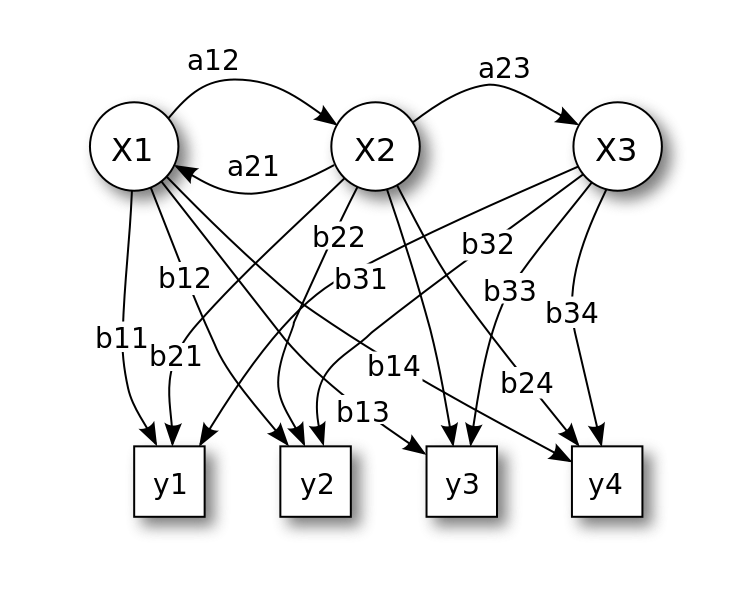
\includegraphics[width=0.6\textwidth]{Bilder/Kap3/hmm_graph.png}
    \caption{Zustandsgraph eines Hidden Markov Models}
    \label{fig:hmm_graph}
\end{figure}


\section{Beispiele}
\textit{ Gefangener im Verlies \footnote{Quelle: \url{http://de.wikipedia.org/wiki/Hidden_Markov_Model}}} \\

\begin{figure}[htbp] \centering
    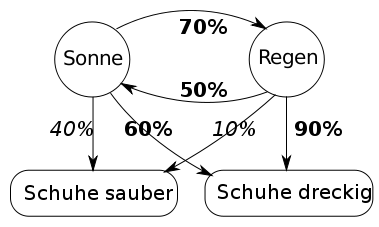
\includegraphics[width=0.4\textwidth]{Bilder/Kap3/hmm_example.png}
    \caption{Hidden Markov Model für das Beipiel des Gefangen im Verlies}
    \label{fig:hmm_example}
\end{figure}

Ein Gefangener im Kerkerverlies möchte das aktuelle Wetter herausfinden. Er weiß, dass auf einen sonnigen Tag zu 70 \% ein Regentag folgt und dass auf einen Regentag zu 50 \% ein Sonnentag folgt. Weiß er zusätzlich, dass die Schuhe der Wärter bei Regen zu 90 \% dreckig, bei sonnigem Wetter aber nur zu 60 \% dreckig sind, so kann er durch Beobachtung der Wärterschuhe Rückschlüsse über das Wetter ziehen (das heißt, er kann die Wahrscheinlichkeit für Regenwetter gegenüber sonnigem Wetter abschätzen). 

Sonne und Regen sind in diesem Fall die versteckten Zustände $x$. Die  Emissionen bzw. die Observation die der Gefangene machen kann sind nur der Verschmutzungsgrad der Schuhe der Wärter $y$. Dabei ist es völlig egal, welches Wetter vor 2 Tage geherrscht hat (Wegen der Markov-Eigenschaft, siehe \ref{sec:mkdef}).

\textit{ Spracherkennung } \\
In der automatischen Spracherkennung entsprechen bspw. die gesprochenen Laute  (Phoneme) den versteckten Zuständen und die Silben bzw. Worte den Emissionen eines Hidden Markov Models (Siehe \cite{speech}). 
Das Model hat somit die Aufgabe, aus einer Sequenz von Lauten auf eine Sequenz von Silben oder Wörtern zu schließen.
Das Hidden Markov Model passt sehr gut zur Vorstellung von Sprachsignalen als Abfolge einzelner Ereignisse.



\section{Definition}
Ein Hidden Markov Model erweitert eine Markov Kette um eine weiteren Zufallsprozess und ist somit ein zweistufiger stochastischer Prozess \cite[67]{mmmFink}. Hierfür wird jedem Zustand der Markov Kette eine Ausgabe bzw. Emission zugeordnet dessen Wahrscheinlichkeitsverteilung einzig vom aktuellen Zustand abhängig ist. Die Emissionen sind die einzigen beobachtbaren Zustände des Hidden Markov Model. Der Rest ist sozusagen 'versteckt' woher sich auch der Name des Models ableitet. Eine Folge von Emissionen wird auch Observationsfolge genannt (Siehe Definition \ref{equ:obs}).
\begin{equation}
\label{equ:obs}
o \in Y; o = y_a, \ldots, y_z
\end{equation}

Das Hidden Markov Model wird in \ref{equ:defhmm} definiert \cite[68]{mmmFink}. 
\begin{equation}
\label{equ:defhmm}
\lambda = (X;Y;A;B;\pi)
\end{equation}
\begin{itemize}
     \item Endlich Menge von Zuständen \\
           \( X = \{ x | 1 <= x <= N \} \)
     \item Alphabeth der Emissionen \\
           \( Y = \{ y | 1 <= y <= M \} \)
     \item Matrix der Zustandsübergangs-wahrscheinlichkeiten \\
           \( A = \{ a_{ij} | a_{ij} = P(X_t = j | X_{t-1} = i) \} \)
     \item Matrix der Emissionsverteilung \\
           \( B = \{ b_{jk} | b_{jk} = P(Y_t = o_k | X_t = j) \} \) bzw. \\
           \( B = \{ b_{j}(x) | b_{j}(x) = p(x|X_t = j) \} \)
     \item Vektor von Zustandsstartwahrscheinlichkeiten \\
           \( \pi = \{ \pi_i | \pi_i = P(X_1 = i) \} \) 
\end{itemize}


Die Emissionsmodellierung ist hierbei vom Kontext der Problemstellung abhängig. Wird das Hidden Markov Model zum Beispiel bei der Analyse von biologischen Sequenzen, spricht von einem diskreten Symbolinventar und es  wird ein diskretes Emissionsmodel genutzt (Siehe Definition \ref{equ:33}). Man spricht hierbei auch von einem diskreten Hidden Markov Model. Wenn dieses Model zur Verarbeitung von Signalen verwendet werden soll, erfordert dies in der Vorverarbeitung der Daten einen Quantisierer der die kontinuerlichen Merkmale in eine diskrete Observationsfolge überführt. 
\begin{equation}
\label{equ:33}
B = \{ b_{jk} | b_{jk} = P(Y_t = o_k | X_t = j) \}
\end{equation}


Gängiger ist es hierfür kontinuierliche Hidden Markov Model's zu nutzen. Hierbei wird eine Emissionsmodelierung auf Basis kontinuierlicher Dichtefunktionen genutzt die kontinuierliche Observationen im \(\mathbb{R}^n\) verarbeitet (Siehe Definition \ref{equ:34}).
\begin{equation}
\label{equ:34}
B =\{ b_{j}(x) | b_{j}(x) = p(x|S_t = j) \}
\end{equation}
Zur Behandlung kontinuerlicher Verteilungen mit mehreren komplexen Häufigkeitsgebieten werden approximatische Verfahren genutzt. Die verbreiteste Technik besteht aus der Verwendung von Mischverteilungen auf der Basis von Gauß-Dichten (Gaussian Mixture Model). Es lässt sich  zeigen, dass sich jede allgemeine kontinuierliche Verteilung \(p(x)\) durch eine Linearkombination von i.a. unendlich vielen Basis-Normalverteilungen beliebig genau approximieren lässt \cite[69]{mmmFink} (Siehe Definition \ref{equ:gmm})
 
\begin{equation}
\label{equ:gmm}
p(x) \hat{=} \sum_{k=1}^\infty c_{k} N(x|\mu_{k},K_{k})\\
\approx \sum_{k=1}^M c_{k} N(x|\mu_{k},K_{k})  
\end{equation}

Der Approximationsgfehler lässt sich hierbei über eine geeignete Anzahl von \(M\) Basisverteilungen klein halten. Somit ergibt sich für die Beschreibung der Emissionsverteilung eines Zustands des Hidden Markov Model folgende Formel:
\begin{equation}
b_{j}(x) = \sum_{k=1}^M c_{jk}g_{jk}(x)
\end{equation}
Die Anzahl der Basisverteilungen eines Gaussian Mixture Model kann hierbei für die einzelnen Zustände des HMM variieren.


\section{Funktionsweise}
Das Konzept des Hidden Markov Model kann laut \cite{rabiner} in drei Problemstellungen eingeteilt werden:
\begin{itemize}
  \item Evaluierungsproblem: Bestimme die Wahrscheinlichkeit für ein Model, mit der dieses eine gegebene Observationsfolge ($o$) erzeugt. (Siehe Abschnitt \ref{sec:eval})
  \item Dekodierungsprobem: Finde interne Abläufe für eine gegebene Observationsfolge (Siehe Abschnitt \ref{sec:decod})
  \item Trainingsproblem: Finde Modellparameter für gegebene Beispieldaten (Siehe Abschnitt \ref{sec:train})
\end{itemize}

\subsection{Evaluierung}
\label{sec:eval}
In der Evaluierung soll die Wahrscheinlichkeit bestimmt werden, mit der eine betrachtete Observationsfolge $o$ in einer beliebigen Zustandsfolge von einem gegebenen Hidden Markov Model $\lambda$ generiert wird. Diese  Wahrscheinlichkeit wird auch Produktionswahrscheinlichkeit genannt. 

Die Produktionswahrscheinlichkeit wird mit dem Forward-Algorithmus berechnet. Der Algorithmus nutzt hierfür die geltende Markov Eigenschaft (Siehe Abschnitt \ref{mainsec:mk}] aus, das nur die Speicherung eines (des letzten) internen Zustandes erlaubt. Hierfür definiert man als Vorwärtsvariable $\alpha_{t}(i)$ die Wahrscheinlichkeit, bei gegebenem Model $\lambda$ den Anfang der betrachteten Observationsfolge $O_{t}$ zu erzeugen und zum Zeitpunkt $t$ den Zustand $i$ zu erreichen (Siehe Definition \ref{equ:eval}).
\begin{equation}
\label{equ:eval}
\alpha_{t}(i) = P(O_{1},O_{2},\ldots,O_{t},s_{t}=i|\lambda)
\end{equation}

Die Vorwährtsvariable lässt sich nun mit den folgenden Schritten rekursiv
berechnen, um dann die Gesamtwahrscheinlichkeit des Models zu erhalten.
\begin{enumerate}
  \item Initialisierung\\
		$\alpha_{1}(i) := \pi_{i}b{i}(O_{1})$
  \item Rekursion\\
	für alle Zeitpunkte $t, t=1 \ldots T-1$\\
	$\alpha_{t+1}(j) :=
	\sum\limits_{i}\{\alpha_{t}(i)\alpha_{ij}\}b_{j}(O_{t+1})$
  \item Rekursionsabschluss\\
  	$P(O|\lambda) = \sum\limits_{i=1}^N \alpha_{T}(i)$
\end{enumerate}


\subsection{Dekodierung}
\label{sec:decod}
Bei der Dekodierung soll, für ein gegebenes $\lambda$ und eine Observationsfolge $o$, die optimale bzw. wahrscheinlichste Zustandsfolge
$s^*$ aus der Menge der Zustände ermittelt werden. Zur Ermittlung der optimalen Zustandsfolge bedient man sich des Viterbi-Algorithmus, einem induktiven Verfahren, dass dem Forward Algorithmus sehr ähnlich ist. Zu Begin werden erneut die Wahrscheinlichkeiten $\delta_{t}(i)$ für partiell optimale Pfade definiert, die das Anfangssegment der Observationsfolge bis $O_{t}$ mit maximaler Wahrscheinlichkeit erzeugen und in Zustand $i$ enden.
\begin{equation}
\delta_{t}(i) =
\max\limits_{s_{1},s_{2}, \ldots
,s_{t}}P(O_{1},\ldots,O_{t},s_{1},\ldots,s_{t}=i|\lambda) 
\end{equation}

Der Algorithmus entspricht weitgehend dem Forward-Algorithmus jedoch werden anstatt der Summe im Rekursionsabschluss, die Maximalen über die in den Vorgängerzuständen vorliegenden Wahrscheinlichkeiten gebildet.
\begin{enumerate}
  \item Initialisierung\\
		\(\delta_{1}(i) := \pi_{i}b{i}(O_{1})\)\\
		\(\phi_{1}(i):=0\)
  \item Rekursion\\
	für alle Zeitpunkte \(t, t=1 \ldots T-1\)\\
	\(\delta_{t+1}(j) :=
	\max\limits_{i}\{\delta_{t}(i)\alpha_{ij}\}b_{j}(O_{t+1})\)\\
	\(\phi_{t+1}(j):= \operatorname{arg\,max}\limits_{i}\{\lambda_{t}(i)\alpha_{ij} \)
  \item Rekursionsabschluss\\
  	\(P^{*}(O|\lambda) = (P(O,s^{*}|\lambda) = \max_{i}\lambda_{T}(i)
  	\alpha_{T}(i)\)
  \item Rückverfolgung des Pfades\\
	für alle Zeitpunkte \(t, t=1 \ldots T-1\)\\
	\(s_{t}^{*}=\phi_{t+1}(s_{t+1}^{*})\)
\end{enumerate}
Mit $\phi_{t}(j)$ wird ein ``Rückwärtszeiger'' definiert, der für jedes
entsprechende $\delta_{t}(j)$ entlang der partiellen Pfade den jeweils
optimalen Vorgängerzustand speichert.


\subsection{Training}
\label{sec:train}
Gegeben sei eine Observationsfolge $o$, aus dem ein passendes Hidden Markov Model erzeugt werden soll. 

Je nach Problemstellung, müssen unterschiedliche Modelle eines HMM's gewählt werden. Es ist bisher kein Verfahren bekannt das aufgrund einer Stichprobe ein optimales Modell generieren kann. Die Anzahl der Zustände, die Wahl der Emissionsverteilungen, sowie deren initiale Parameterwerte müssen nach eigenen Erfahrungen gewählt werden. Wenn dies geschehen ist kann das Modell in einem iterativen Prozess trainiert werden. Hierbei werden die Parameter einer Wachstumstransformation unterworfen. Ziel ist es das die Modellparameter so verändert werden, dass die Bewertung des veränderten Models besser, als die des Ausgangsmodels ist.

Zum trainieren eines Hidden Markov Model existieren diverse Algorithmen. Sie unterscheiden sich im wesentlichen durch die Verwendeten Qualitätsmaße zur Bewertung der Modelierungsgüte. Beim Baum-Welch-Algorithmus \cite{rabiner} wird die Produktionswahrscheinlichkeit \(P(O|\lambda)\) zur Bewertung genutzt. Beim Viterbi-Algorithmus \cite{viterbi} und dem eng verwandten Segmental-k-means Algorithmus \cite{juang} nur die Wahrscheinlichkeit \((P(O,s^{*}|\lambda)\) der jeweils optimalen Zustandsfolge betrachtet \cite{mmmFink}.
